\chapter[Appendix]{Appendix} \label{ch:appendix}

Due to unknown technical issues, it seems that the SOLiD sequencer has some problems recovering the CpG islands from the genome. We experienced repeated failure of performing FOXM1 ChIP-seq experiments using the SOLiD platform. The problems do not seem to be the library preparation, since good fold enrichments on target genes can be detected both before and after the library preparation (\textbf{Figure \ref{fig:fig57}A}). By using the Illumina platform, FOXM1 ChIP-seq experiments were successfully done without any problems.

When comparing the binding profiles of the FOXM1 ChIP-seq experiments from SOLiD and Illumina, SOLiD fails to recover all the 270 peaks which are detected by both Illumina platform and ChIP-qPCR (\textbf{Figure \ref{fig:fig57}B}).

\begin{figure}[!h]
    \centering
    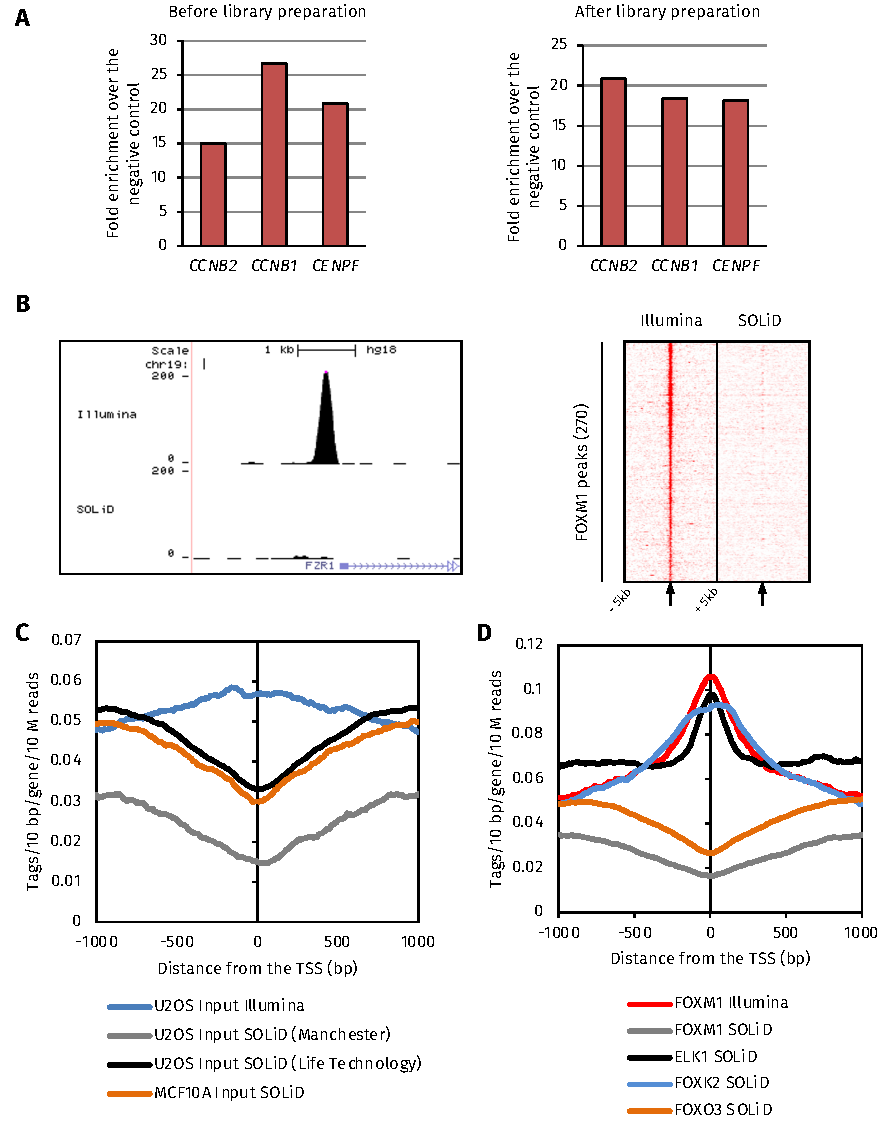
\includegraphics[width=0.9\textwidth]{appendix/figures/fig57.pdf}
    \caption[Examples of technical issues of the SOLiD platform]{\textbf{Examples of technical issues of the SOLiD platform. (A)} ChIP-qPCR on the indicated FOXM1 target genes before (left) and after (right) the library preparation for the SOLiD platform. Fold enrichments over the \textit{PLK1} negative region are shown. \textbf{(B) Left,} an example of the Illumina profile (top) and the SOLiD profile (bottom) at the \textit{FZR1} locus. \textbf{Right,} heatmap of tag density profiles of FOXM1 ChIP-seq tags from the Illumina and the SOLiD platforms around the 270 peaks of FOXM1. Tags were calculated in every 50 bp bin, and the density profiles were normalised to tags per 10 million total reads per bin. The middle point of each panel (indicated by small arrows below) represents the summit of the FOXM1 peak generated using the Illumina platform. 5 kb upstream and 5 kb downstream around the summit were plotted. \textbf{(C)} Quantification of average tags around the transcription start sties (TSS) of all RefSeq genes. Genes were aligned by their TSS, and the region of -1000 and +1000 bp relative to the TSS was selected. Tags were calculated in every 10 bp bin and normalised to tags per 10 million total reads per bin per gene. \textbf{(D)} The same analysis as \textbf{(C)} but using the reads from the indicated ChIP samples and different sequencing platforms.}
    \label{fig:fig57}
\end{figure}

When aligning the reads from input samples to the transcription start sites of all Refseq annotated genes, which ideally should be uniformly distributed, the input sample from the Illumina platform has a slight enrichment around the TSS (\textbf{Figure \ref{fig:fig57}C}, the blue line), which is a common phenomenon in ChIP-seq studies (\cite{auerbach2009mapping,cheung2011systematic}), presumably because many TSS regions are located within open chromatin regions which tend to get higher coverage (see \textbf{Section \ref{section:chiplimitation}}). Surprisingly, the input sample from the SOLiD platform from our core facility exhibits a \enquote{dip} in tag density around the TSS regions (\textbf{Figure \ref{fig:fig57}C}, the grey line). This is not a specific issue from this study, because an input sample of MCF10A cells from another experiment (\cite{odrowaz2012elk1}) also shows a similar depletion of reads around the TSS regions (\textbf{Figure \ref{fig:fig57}C}, the orange line). This is not a specific issue from our core facility either, because our FOXK2 ChIP- seq data was done at a facility from Life Technology, and the input sample from the FOXK2 ChIP-seq data also exhibits a \enquote{dip} in tag density around the TSS regions (\textbf{Figure \ref{fig:fig57}C}, the black line).

When aligning the reads from FOXM1 ChIP samples to the transcription start sites, the sample from the Illumina platform exhibits a nice enrichment in tag density around the TSS regions of all Refseq annotated genes (\textbf{Figure \ref{fig:fig57}D}, the red line), which is consistent with its experimental validation. In contrast, the sample from the SOLiD platform, again, shows a \enquote{dip} in tag density around the TSS regions (\textbf{Figure \ref{fig:fig57}D}, the grey line). This seems to be a specific problem for FOXM1, because FOXK2 and ELK1 (both from the SOLiD platform) show good enrichments surrounding the TSS regions (\textbf{Figure \ref{fig:fig57}D}, the blue and the black lines). Interestingly, FOXO3 ChIP signals (SOLiD platform) also displays a depletion of reads near the TSS regions (\textbf{Figure \ref{fig:fig57}D}, the orange line).

It seems that the SOLiD platform is able to detect some binding events near promoters as demonstrated by ELK1 which also tends to bind promoter regions (\cite{odrowaz2012elk1}). We next noticed that 77\% FOXM1 binding events overlap with the CpG islands, while 46\% ELK1 binding sites are within the CpG islands, and only 2.5\% and 10.3\% FOXK2 and FOXO3 peaks overlap with the CpG islands respectively. Therefore, we suspect that the SOLiD platform may have problems recovering the CpG islands from the genome.

Since the FOXM1 ChIP-seq experiments failed in the SOLiD platform, the comparisons between different sequencing platforms using the FOXM1 data might not be appropriate. To gain a preliminary idea about the potential differences between the Illumina and SOLiD sequencing platforms, we used our FOXK2 ChIP-seq data which were performed on both the SOLiD and the Illumina platforms at the same time, and both platforms successfully identified similar numbers of FOXK2 binding peaks.

\begin{figure}[!h]
    \centering
    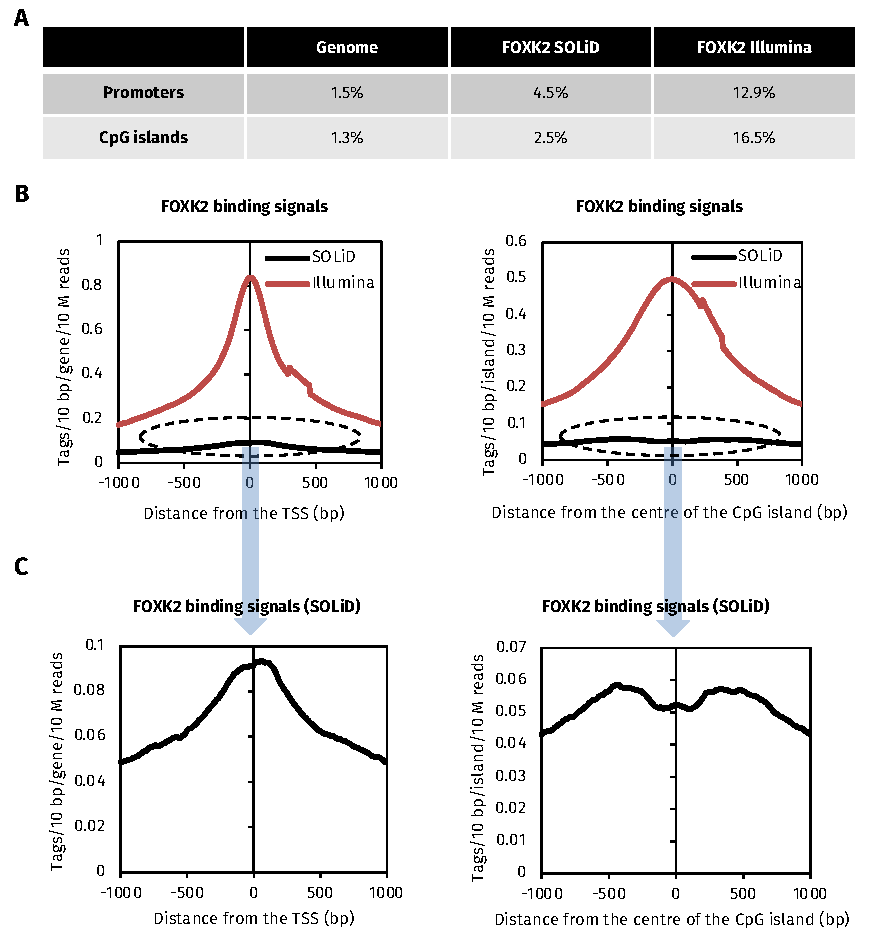
\includegraphics[width=0.9\textwidth]{appendix/figures/fig58.pdf}
    \caption[Comparisons between the FOXK2 ChIP-seq data from the Illumina and the SOLiD platforms]{\textbf{Comparisons between the FOXK2 ChIP-seq data from the Illumina and the SOLiD platforms. (A)} Percentages of peaks distributions identified from different platforms. The genome background is also shown. The promoter region was defined as 5'- UTR and up to 1000 bp upstream from the TSS. \textbf{(B)} Quantification of average tags from the Illumina platform (the red line) and the SOLiD platform (the black line) around the TSS of all RefSeq genes (left) and the CpG islands (right). Genes were aligned by their TSS and the CpG islands were aligned by their mid point. The region of -1000 and +1000 bp relative to the TSS or the centre of the CpG islands was selected. Tags were calculated in every 10 bp bin and normalised to tags per 10 million total reads per bin per region. \textbf{(C)} The same analysis as \textbf{(B)} but only using the reads from the SOLiD sequencing platforms.}
    \label{fig:fig58}
\end{figure}

First, we checked the genomic distributions of FOXK2 peaks identified from the SOLiD and the Illumina platforms respectively. Higher percentage of peaks from the Illumina platform were located in the promoter regions (\textbf{Figure \ref{fig:fig58}A}), while the distributions of peaks at other locations were relatively similar (data not shown). When compared to the overlap with CpG islands, the difference between the peaks from the two platforms was even more prominent (\textbf{Figure \ref{fig:fig58}A}). Next, we checked the FOXK2 ChIP signals around either the TSS regions or the CpG islands. The signals from the Illumina platform were much higher than those from the SOLiD platform in both cases (\textbf{Figure \ref{fig:fig58}B}), indicating SOLiD platform has a problem recovering the signals from these regions. When looked into the detail of the ChIP signals from the SOLiD platform, FOXK2 still showed a slight enrichment around the TSS regions (\textbf{Figure \ref{fig:fig58}C}, left panel), but there was a \enquote{dip} in tag density of FOXK2 around the CpG islands (\textbf{Figure \ref{fig:fig58}C}, right panel). Therefore, we suspect that the SOLiD platform may have problems recovering the CpG islands from the genome.

Considering the limitations of the SOLiD platform, the overlap between FOXK2, FOXO3 and FOXM1 presented in this study might be an underestimation. The binding of FOXK2 and FOXO3 to the promoter regions might be underestimated as well. However, since direct comparisons between FOXK2 and FOXO3 are performed within the same platform, we argue that the overall conclusions should not be greatly affected.